
\iffalse
%%%%%%%%%%%%%%%%%%%%%%%%%%%%%%%%%%%%%%%%%%%%%%%%%%%%%%%%%%%%%%%%%%%%%%%%
%
% This is the template file for the 6th International conference
% NONLINEAR ANALYSIS AND EXTREMAL PROBLEMS
% June 25-30, 2018
% Irkutsk, Russia
%
%%%%%%%%%%%%%%%%%%%%%%%%%%%%%%%%%%%%%%%%%%%%%%%%%%%%%%%%%%%%%%%%%%%%%%%%
% The preparation of the article is based on the standard llncs class
% (Lecture Notes in Computer Sciences), which is adjusted with style
% file of the conference.
%
% There are two ways of compilation of the file into PDF
% 1. Use pdfLaTeX (pdflatex), (LaTeX+DVIPS will not work);
% 2. Use LuaLaTeX (XeLaTeX will work too).
% When using LuaLaTeX You will need TTF or OTF CMU fonts
% (Computer Modern Unicode). The fonts are installed with 'cm-unicode' package in
% a distribution of LaTeX % (https://www.ctan.org/tex-archive/fonts/cm-unicode),
% either by downloading and installing these fonts system wide, the address of their page is
% http://canopus.iacp.dvo.ru/%7Epanov/cm-unicode/
% The second option won't work in XeLaTeX.
%
% For MiKTeX (LaTeX distribution for Windows),
%  1. Package 'cm-unicode' is installed manually with the MiKTeX administration Console.
%  2. For the compilation of this example, namely, the stub figure, one will also need to
% download package 'pgf' manually. This package uses in the popular
% package tikz.
%  3. Tests showed that the rest of the required packages MiKTeX loads automatically (if
%     it is allowed). The 'auto download' option is
%     configured in 'Settings' section in MiKTeX Console.
%
%
% The easiest way to compile an article is to use pdfLaTeX, but
% the final layout of the book will be compiled with LuaLaTeX,
% as a result will be of better quality thanks to the package 'microtype' and
% use vector OTF instead of standard raster fonts of pdfLaTeX.
%
% In the case of questions and problems with the article compilation,
% write letters to e-mail: eugeneai@irnok.net, Cherkashin Evgeny.
%
% New version of the correcting style file will be available at the website:
%     https://github.com/eugeneai/nla-style
%     file - nla.sty
%
% Further instructions are in the text body of the template. The template itself
% is an article example.
%
% The LaTeX2e format is used!

% 12 points font size is used.
\documentclass[12pt]{llncs}

% The correcting style file is added.
\usepackage{todonotes}

\usepackage{nla} % This package is needed for compiling
                 % this template, it should be removed
                 % from your article.

% Many popular packages (amsXXX, graphicx, etc.) are already imported in the style file.
% If there is a conflict with your packages, try disabling them and compile
% the text.
%
% It would be convenient in the layout of the proceedings if the file names
% of the figures of different authors do not clash.
% To minimize the clash, the drawings can be placed in a separate subfolder
% named after the author or the title of the paper.
%
% \graphicspath{{ivanov-petrov-pics/}} % specifies the folder with images in png, pdf formats.
% or
% \graphicspath{{great-problem-solving-paper-pics/}}.

%\usepackage{float}
\begin{document}
\fi
% Text should be formatted in accordance with the 'article' class, using extensions like
% AMS.
%
\title{The effects of viscous dissipation on the nanofluid natural convection in a tilted square cavity\thanks{The research is supported by partially by the  Natural Science Foundation of Liaoning Province in China, project No.~2022-BS-093, the  Fundamental Research Funds for the Central Universities of China, project No.~3132023203 and  the Educational Science Planning Projects of Liaoning Province of China, project No.~JG21DB065. }}
% First author
\author{Longjie Lv\inst{1} \and Shuguang Li\inst{2} \and  Mingyue Wei\inst{3}
}
\institute{School of Science, Dalian Maritime University, Dalian,  China\\
  \email{1783572186qq@dlmu.edu.cn}
  \and
School of Science, Dalian Maritime University, Dalian,  China\\
\email{shuguangli2008@126.com}
\and
School of Science, Dalian Maritime University, Dalian,  China\\
\email{w15633860221@163.com}}
% etc

\maketitle

\begin{abstract}
The viscous dissipation  leads to changes in the temperature, viscosity, heat transfer and other physical properties of the fluid during the flow process, thereby affecting the flow characteristics.
And it plays an important role in damping effect, momentum transfer and energy dissipation. Therefore, more in-depth research is needed to reveal the importance of viscous dissipation in natural convection.
In this work, the effects of viscous dissipation on the flow and heat transfer of nanofluid natural convection in a tilted square cavity are numerically studied by applying a newly proposed fractional-step semi-implicit algorithm with the numerical advantage of larger time steps. The cavity is filled with water and nanoparticles of copper ($Cu$), and the viscous dissipative behavior of the mixture flow is not negligible. This study has been conducted for certain pertinent parameters of Rayleigh number ($Ra = 10^{4}$ and $10^{5}$), Prandtl number ($Pr = 6.2$), Eckert number ($Ec$ = 0 $-$ 2), the volume fraction of solid particles ($\phi$ = 0 $-$ 0.06), and inclination angle of square cavity ($\alpha$ = 0 $-$ $\pi/2$).
\keywords{Natural convection,  Heat transfer, Nanofluid, Viscous dissipation, Fractional-step semi-implicit algorithm.}
\end{abstract}

% at the end of the list, there should be no final dot
%\section{The main results}


The results show that at any tilt angle , the increase in viscous dissipation leads to weakened heat transfer on the hot wall, enhanced heat transfer on the cold wall, and weakened flow in the square cavity. Adding solid particles can effectively weaken the effect of viscous dissipation. As the Rayleigh number increases, the effect of viscous dissipation increases. As the tilt angle increases, the effects of volume fraction and Eckert number weaken.

% The figures and tables are drawn according to the standard class 'article'.
\begin{figure}[htb]
 \centering
\vspace{-4cm}  
\setlength{\abovecaptionskip}{-3.cm}  
%% Two picture formats are supported:
\includegraphics[width=0.48\linewidth]{1.eps} % Raster format
\includegraphics[width=0.48\linewidth]{2.eps} % Vector and raster format
\caption{The effect of Eckert number on the average Nusselt number $Nu_{0}$ on the hot wall and the average Nusselt number $Nu_{1}$ on the cold wall with different volume fractions of the solid particles $\phi$ in a horizontally placed square cavity($\alpha$ = 0) at $Ra$ = $10^{5}$ }
%
% Vector drawings can be drawn in Inkscape editor
% https://inkscape.org/ru/download/
% The usual format of the editor is SVG, so the drawings must be exported in
% PDF or PNG (with a resolution of minimum 150 dpi, and maximum of 300 dpi).
  %\begin{center}
   % \missingfigure[figwidth=0.7\linewidth]{Remove me from the article!} \end{center}
  %\caption{Caption of the figure}\label{fig:example}
\end{figure}
The numerical results in Fig 1 show that for any solid particle volume fraction, viscous dissipation leads to reduced heat transfer on the hot wall and enhanced heat transfer on the cold wall. And as the volume fraction of solid particles increases, the effect of Eckert number on  heat transfer weakens.
\begin{figure}[htb]
 \centering
\vspace{-3.5cm}   
\setlength{\abovecaptionskip}{-3.cm}  
%% Two picture formats are supported:
\includegraphics[width=0.48\linewidth]{3.eps} % Raster format
\includegraphics[width=0.48\linewidth]{4.eps} % Vector and raster format
\caption{The effect of inclination angle $\alpha$ on the average Nusselt number $Nu_{0}$ on the hot wall and the average Nusselt number $Nu_{1}$ on the cold wall at $Ra$ = $10^{5}$}
%
% Vector drawings can be drawn in Inkscape editor
% https://inkscape.org/ru/download/
% The usual format of the editor is SVG, so the drawings must be exported in
% PDF or PNG (with a resolution of minimum 150 dpi, and maximum of 300 dpi).
  %\begin{center}
   % \missingfigure[figwidth=0.7\linewidth]{Remove me from the article!} \end{center}
  %\caption{Caption of the figure}\label{fig:example}
\end{figure}
The numerical results in Fig 2 show that as the tilt angle increases, the effects of solid particle volume fraction and Eckert number weaken.
% At the end of the text, acknowledgments are expressed, if you haven't
% made a footnote from the title. For example, we can write

\begin{thebibliography}{9} % or {99}, if there is more than ten references.
\bibitem{LiLv2024} Li S.G., Lv L.J., Liao M.Y. Numerical simulation of heat transfer and entropy generation due to the nanofluid natural convection with viscous dissipation in an inclined square cavity. Numer. Heat Transf. A Appl.~2024. https://doi.org/10.1080/10407782.2024.2325121

\bibitem{LiFu2023} Li S.G., Fu H.S. A new high-order compact and conservative numerical scheme for the generalized symmetric regularized long wave equations. Int. J. Comput. Math.~2023. Vol.~100, no~5. Pp.~968--990. https://doi.org/10.1080/00207160.2023.2167516

\bibitem{DiLi2020} Dimitrienko Y.I., Li S.G. Numerical simulation of MHD natural convection heat transfer in a square cavity filled with Carreau fluids under magnetic fields in different directions. Comput. Appl. Math.~2020. Vol.~39, no~4. Pp.~252. https://doi.org/10.1007/s40314-020-01300-w

%\bibitem{Ke2016}  Kefayati G.H.R. Simulation of heat transfer and entropy generation of MHD natural convection of non-Newtonian nanofluid in an enclosure. Int J Heat Mass Tran.~2016. Vol.~92. Pp.~1066--1089.

%\bibitem{Zh2012} Zhang K., Yang M., Zhang Y. A compact finite-difference scheme based on the projection method for natural-convection heat transfer. Numer Heat Tr B-Fund.~2012. Vol.~61, no~4. Pp.~259--278.

%\bibitem{1983} de Vahl Davis G. Natural convection of air in a square cavity: a bench mark numerical solution. Int J Numer Meth Fl.~1983. Vol.~3, no~3. Pp.~249--264.

%\bibitem{Ch1968} Chorin A.J. Numerical solution of the Navier-Stokes equations.
%Math Comput.~1968. Vol.~22, no~104. Pp.~745--762.

\end{thebibliography}
%\end{document}